\documentclass[]{article}
\usepackage{lmodern}
\usepackage{amssymb,amsmath}
\usepackage{ifxetex,ifluatex}
\usepackage{fixltx2e} % provides \textsubscript
\ifnum 0\ifxetex 1\fi\ifluatex 1\fi=0 % if pdftex
  \usepackage[T1]{fontenc}
  \usepackage[utf8]{inputenc}
\else % if luatex or xelatex
  \ifxetex
    \usepackage{mathspec}
  \else
    \usepackage{fontspec}
  \fi
  \defaultfontfeatures{Ligatures=TeX,Scale=MatchLowercase}
\fi
% use upquote if available, for straight quotes in verbatim environments
\IfFileExists{upquote.sty}{\usepackage{upquote}}{}
% use microtype if available
\IfFileExists{microtype.sty}{%
\usepackage{microtype}
\UseMicrotypeSet[protrusion]{basicmath} % disable protrusion for tt fonts
}{}
\usepackage[margin=1in]{geometry}
\usepackage{hyperref}
\hypersetup{unicode=true,
            pdftitle={Study Verification Test},
            pdfborder={0 0 0},
            breaklinks=true}
\urlstyle{same}  % don't use monospace font for urls
\usepackage{longtable,booktabs}
\usepackage{graphicx,grffile}
\makeatletter
\def\maxwidth{\ifdim\Gin@nat@width>\linewidth\linewidth\else\Gin@nat@width\fi}
\def\maxheight{\ifdim\Gin@nat@height>\textheight\textheight\else\Gin@nat@height\fi}
\makeatother
% Scale images if necessary, so that they will not overflow the page
% margins by default, and it is still possible to overwrite the defaults
% using explicit options in \includegraphics[width, height, ...]{}
\setkeys{Gin}{width=\maxwidth,height=\maxheight,keepaspectratio}
\IfFileExists{parskip.sty}{%
\usepackage{parskip}
}{% else
\setlength{\parindent}{0pt}
\setlength{\parskip}{6pt plus 2pt minus 1pt}
}
\setlength{\emergencystretch}{3em}  % prevent overfull lines
\providecommand{\tightlist}{%
  \setlength{\itemsep}{0pt}\setlength{\parskip}{0pt}}
\setcounter{secnumdepth}{0}
% Redefines (sub)paragraphs to behave more like sections
\ifx\paragraph\undefined\else
\let\oldparagraph\paragraph
\renewcommand{\paragraph}[1]{\oldparagraph{#1}\mbox{}}
\fi
\ifx\subparagraph\undefined\else
\let\oldsubparagraph\subparagraph
\renewcommand{\subparagraph}[1]{\oldsubparagraph{#1}\mbox{}}
\fi

%%% Use protect on footnotes to avoid problems with footnotes in titles
\let\rmarkdownfootnote\footnote%
\def\footnote{\protect\rmarkdownfootnote}

%%% Change title format to be more compact
\usepackage{titling}

% Create subtitle command for use in maketitle
\newcommand{\subtitle}[1]{
  \posttitle{
    \begin{center}\large#1\end{center}
    }
}

\setlength{\droptitle}{-2em}
  \title{Study Verification Test}
  \pretitle{\vspace{\droptitle}\centering\huge}
  \posttitle{\par}
  \author{}
  \preauthor{}\postauthor{}
  \date{}
  \predate{}\postdate{}


\begin{document}
\maketitle

Campus: AAL

Student: Mike Eistrup Poulsen

\subsection{Student Report}\label{student-report}

This is an interpretive report of your responses to the Study
Verification Test. Its purpose is to help you identify your student
profile within specific topics.

The percentile ranks show how you compare to a larger sample of first
semester Medialogy students from Aalborg and Copenhagen. Specifically,
they indicate the percentage of students whose scores are equal to or
less than yours. The percentile is also indicated with a dot in the
boxplots where the x-axis show the number of standard deviations away
from the mean (indicated with a grey line at 0).

As the report is based on questionnaire information alone, it may give
only a rough indication of your true attitudes. Your advisor or
counselor will help you understand your scores and find the services you
desire.

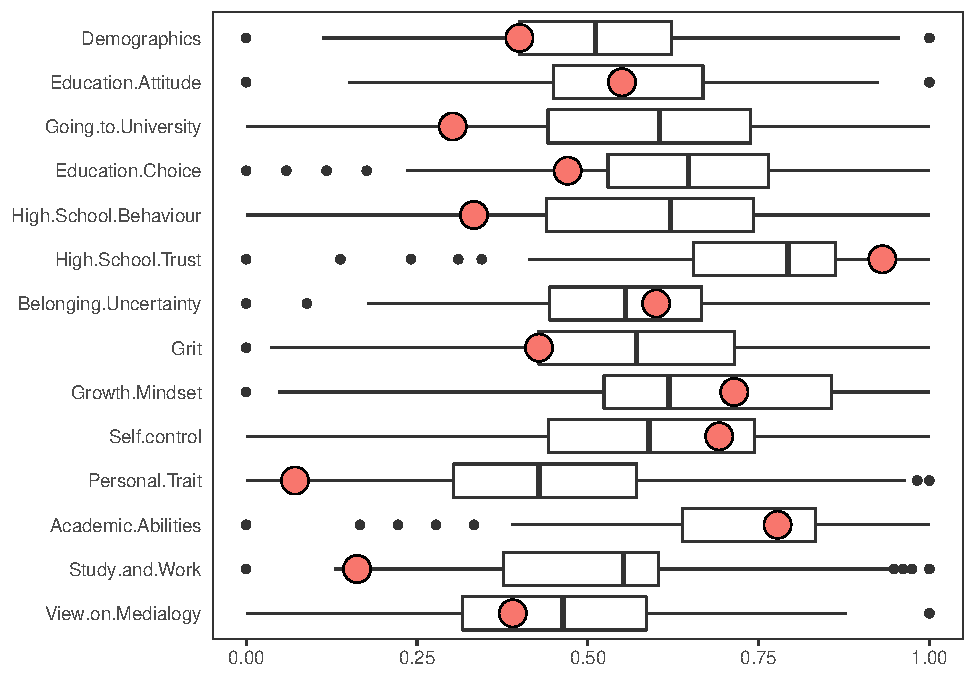
\includegraphics{C:/Users/BiancaClavio/Documents/stats-on-grades/docs/handouts/SSPanalysis_8_files/figure-latex/unnamed-chunk-2-1.pdf}

\begin{longtable}[]{@{}llr@{}}
\toprule
variable & Scaled avg. score & Percentile rank\tabularnewline
\midrule
\endhead
Demographics & -1.62007029 & 0\tabularnewline
Education.Attitude & -2.31996412 & 0\tabularnewline
Going.to.University & -0.85986843 & 0\tabularnewline
Education.Choice & -1.13172600 & 0\tabularnewline
High.School.Behaviour & -2.48630768 & 0\tabularnewline
High.School.Trust & -1.52177107 & 0\tabularnewline
Belonging.Uncertainty & -1.92103827 & 0\tabularnewline
Grit & -1.62096319 & 0\tabularnewline
Growth.Mindset & -0.37024287 & 0\tabularnewline
Self.control & 0.25955451 & 0\tabularnewline
Personal.Trait & -1.16556829 & 0\tabularnewline
Academic.Abilities & -0.03183118 & 0\tabularnewline
Study.and.Work & 0.83016368 & 0\tabularnewline
View.on.Medialogy & -0.96252314 & 0\tabularnewline
\bottomrule
\end{longtable}


\end{document}
